\documentclass[11pt,a4paper]{article}
\usepackage{geometry}
\geometry{margin=1in}
\usepackage{amsmath}
\usepackage{graphicx}
\usepackage{caption}
\usepackage{subcaption}
\usepackage{hyperref}
\usepackage{listings}
\usepackage[utf8]{inputenc}
\usepackage{float}
\lstset{
  basicstyle=\ttfamily\small,
  numbers=left,
  numberstyle=\tiny,
  stepnumber=1,
  numbersep=5pt,
  frame=single,
  breaklines=true,
  captionpos=b
  iterate={&}{{\&}}1 {·}{}1 {_}{{\_}}1
}
\title{Dissipative Particle Dynamics Simulations\\\large Homework 4 Report}
\author{Zitian Wang}
\date{April 30, 2025}

\begin{document}
\maketitle

\begin{abstract}
In this work, we perform 2D DPD simulations for three cases: pure fluid equilibrium, Couette flow with chain molecules, and Poiseuille flow with ring molecules. We validate temperature control, analyze velocity profiles, and study molecular conformation and migration under flow.
\end{abstract}

\section{Introduction}
DPD combines conservative, dissipative, and random forces to model mesoscopic fluids. We examine:
\begin{itemize}
  \item Pure fluid: temperature stability and velocity distribution.
  \item Couette flow: shear-induced chain stretching and velocity profiles.
  \item Poiseuille flow: pressure-driven ring migration and concentration profiles.
\end{itemize}

\section{Model and Methods}
\subsection{Simulation Domain and Boundaries}
A square domain of side $L=15$ with periodic boundaries. Solid walls of width $r_c=1$ at $y<r_c$ and $y>L-r_c$. In Couette, walls move at $\pm5$; in Poiseuille, walls are fixed and a constant body force $F_{body}=0.3$ drives flow.

\subsection{DPD Force Model}
Interparticle forces are:\
\begin{align*}
F^C_{ij}&=a_{ij}\,(1-\tfrac{r_{ij}}{r_c})\,\hat r_{ij},\\
F^D_{ij}&=-\gamma\,w_D(r_{ij})(\hat r_{ij}\cdot v_{ij})\hat r_{ij},\\
F^R_{ij}&=\sigma\,w_R(r_{ij})\,\xi_{ij}\hat r_{ij}/\sqrt{\Delta t},
\end{align*}
with $\gamma=4.5$, $\sigma=\sqrt{2\gamma k_BT}=\sqrt{9}$, $k_BT=1$. Bond forces use harmonic springs: $F^S_{ij}=K_S(1- r_{ij}/r_S)\hat r_{ij}$.

\subsection{Key Implementation Snippets}
Domain and parameters:
\begin{lstlisting}[caption={Global Constants and Parameter Choices}]
L = 15.0           # Domain size
rc = 1.0           # Cutoff radius
rho = 4.0          # Fluid number density
DT = 0.001         # Time step
mass = 1.0
gamma = 4.5
kT = 1.0
sigma = np.sqrt(2*gamma*kT)  # noise amplitude
cell_size = rc
\end{lstlisting}

Cell-list construction:
\begin{lstlisting}[caption={build\_cell\_list (neighbor search)}]
def build_cell_list(pos):
    n = int(np.floor(L / cell_size))
    head   = -np.ones((n,n), dtype=np.int32)
    linked = -np.ones(pos.shape[0], dtype=np.int32)
    for i in range(pos.shape[0]):
        cx = int(pos[i,0]/cell_size) % n
        cy = int(pos[i,1]/cell_size) % n
        linked[i] = head[cx,cy]
        head[cx,cy] = i
    return head, linked, n
\end{lstlisting}

Integrator (velocity-Verlet):
\begin{lstlisting}[caption={integrate (Velocity-Verlet step)}]
@njit
def integrate(pos, vel, acc):
    for i in range(pos.shape[0]):
        vel[i] += 0.5 * acc[i] * DT
        pos[i] += vel[i] * DT
        # periodic wrap
        for d in range(2):
            if pos[i,d] >= L: pos[i,d] -= L
            if pos[i,d] <  0: pos[i,d] += L
\end{lstlisting}

Molecule and wall initialization:
\begin{lstlisting}[caption={create\_chain, create\_ring, create\_walls}]
def create_chain(n):
    # positions, types, bonds for linear chains
    ...

def create_ring(n):
    # positions, types, bonds for ring molecules
    ...

def create_walls(mode):
    # positions, types, and velocities for walls
    ...
\end{lstlisting}

Force computation snippet is shown below:
\begin{lstlisting}[caption={compute\_dpd\_forces (DPD force model)}]
@njit
def compute_dpd_forces(pos, vel, acc, ptype, head, linked, n_cells, aij):
    acc[:,:] = 0.0
    sqrt_dt = np.sqrt(DT)
    for i in prange(pos.shape[0]):
        ...
\end{lstlisting}

\section{Simulation Setup and Data Storage}
Each case saves data to a compressed NPZ file:
\begin{lstlisting}[caption={Data saving example}]
np.savez_compressed(
  'data/couette/couette.npz',
  yedges=yedges, steps=steps_c, temps=temps_c,
  vprofs=vprofs, e2es=e2es
)
\end{lstlisting}

\section{Results and Analysis}
\subsection{Pure Fluid Test}
Figure~\ref{fig:pre_temp} shows temperature vs step, omitting initial 1000 steps to avoid transient spikes.
\begin{figure}[h]
  \centering
  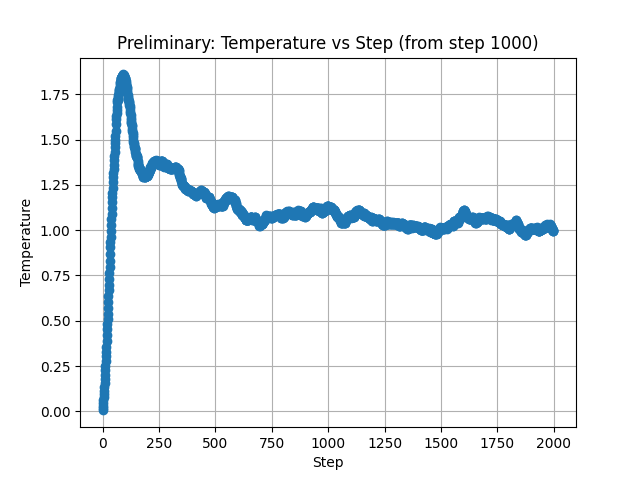
\includegraphics[width=0.7\textwidth]{figures/preliminary/temperature_vs_step.png}
  \caption{Temperature evolution (steps $\ge1000$). Stabilizes at $T\approx1$.}
  \label{fig:pre_temp}
\end{figure}
The system exhibits rapid equilibration and maintains the target temperature, indicating correct thermostat implementation.

Figure~\ref{fig:pre_speed} displays the speed distribution after equilibrium, matching the Maxwell–Boltzmann form.
\begin{figure}[h]
  \centering
  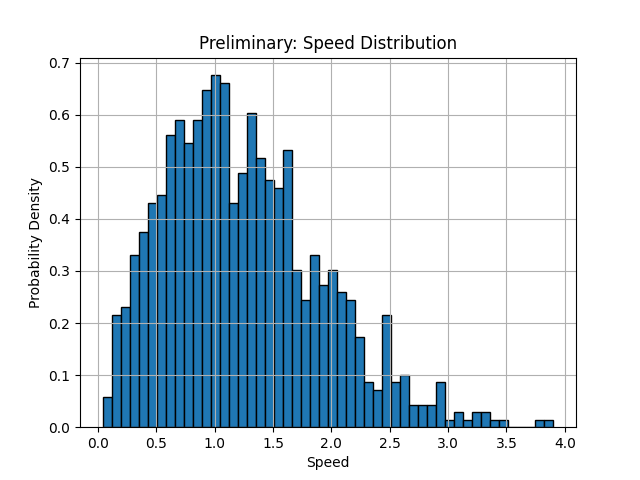
\includegraphics[width=0.7\textwidth]{figures/preliminary/speed_distribution.png}
  \caption{Velocity magnitude distribution after equilibration.}
  \label{fig:pre_speed}
\end{figure}

% Time-step dependence figure inserted with fixed placement
\begin{figure}[H]
  \centering
  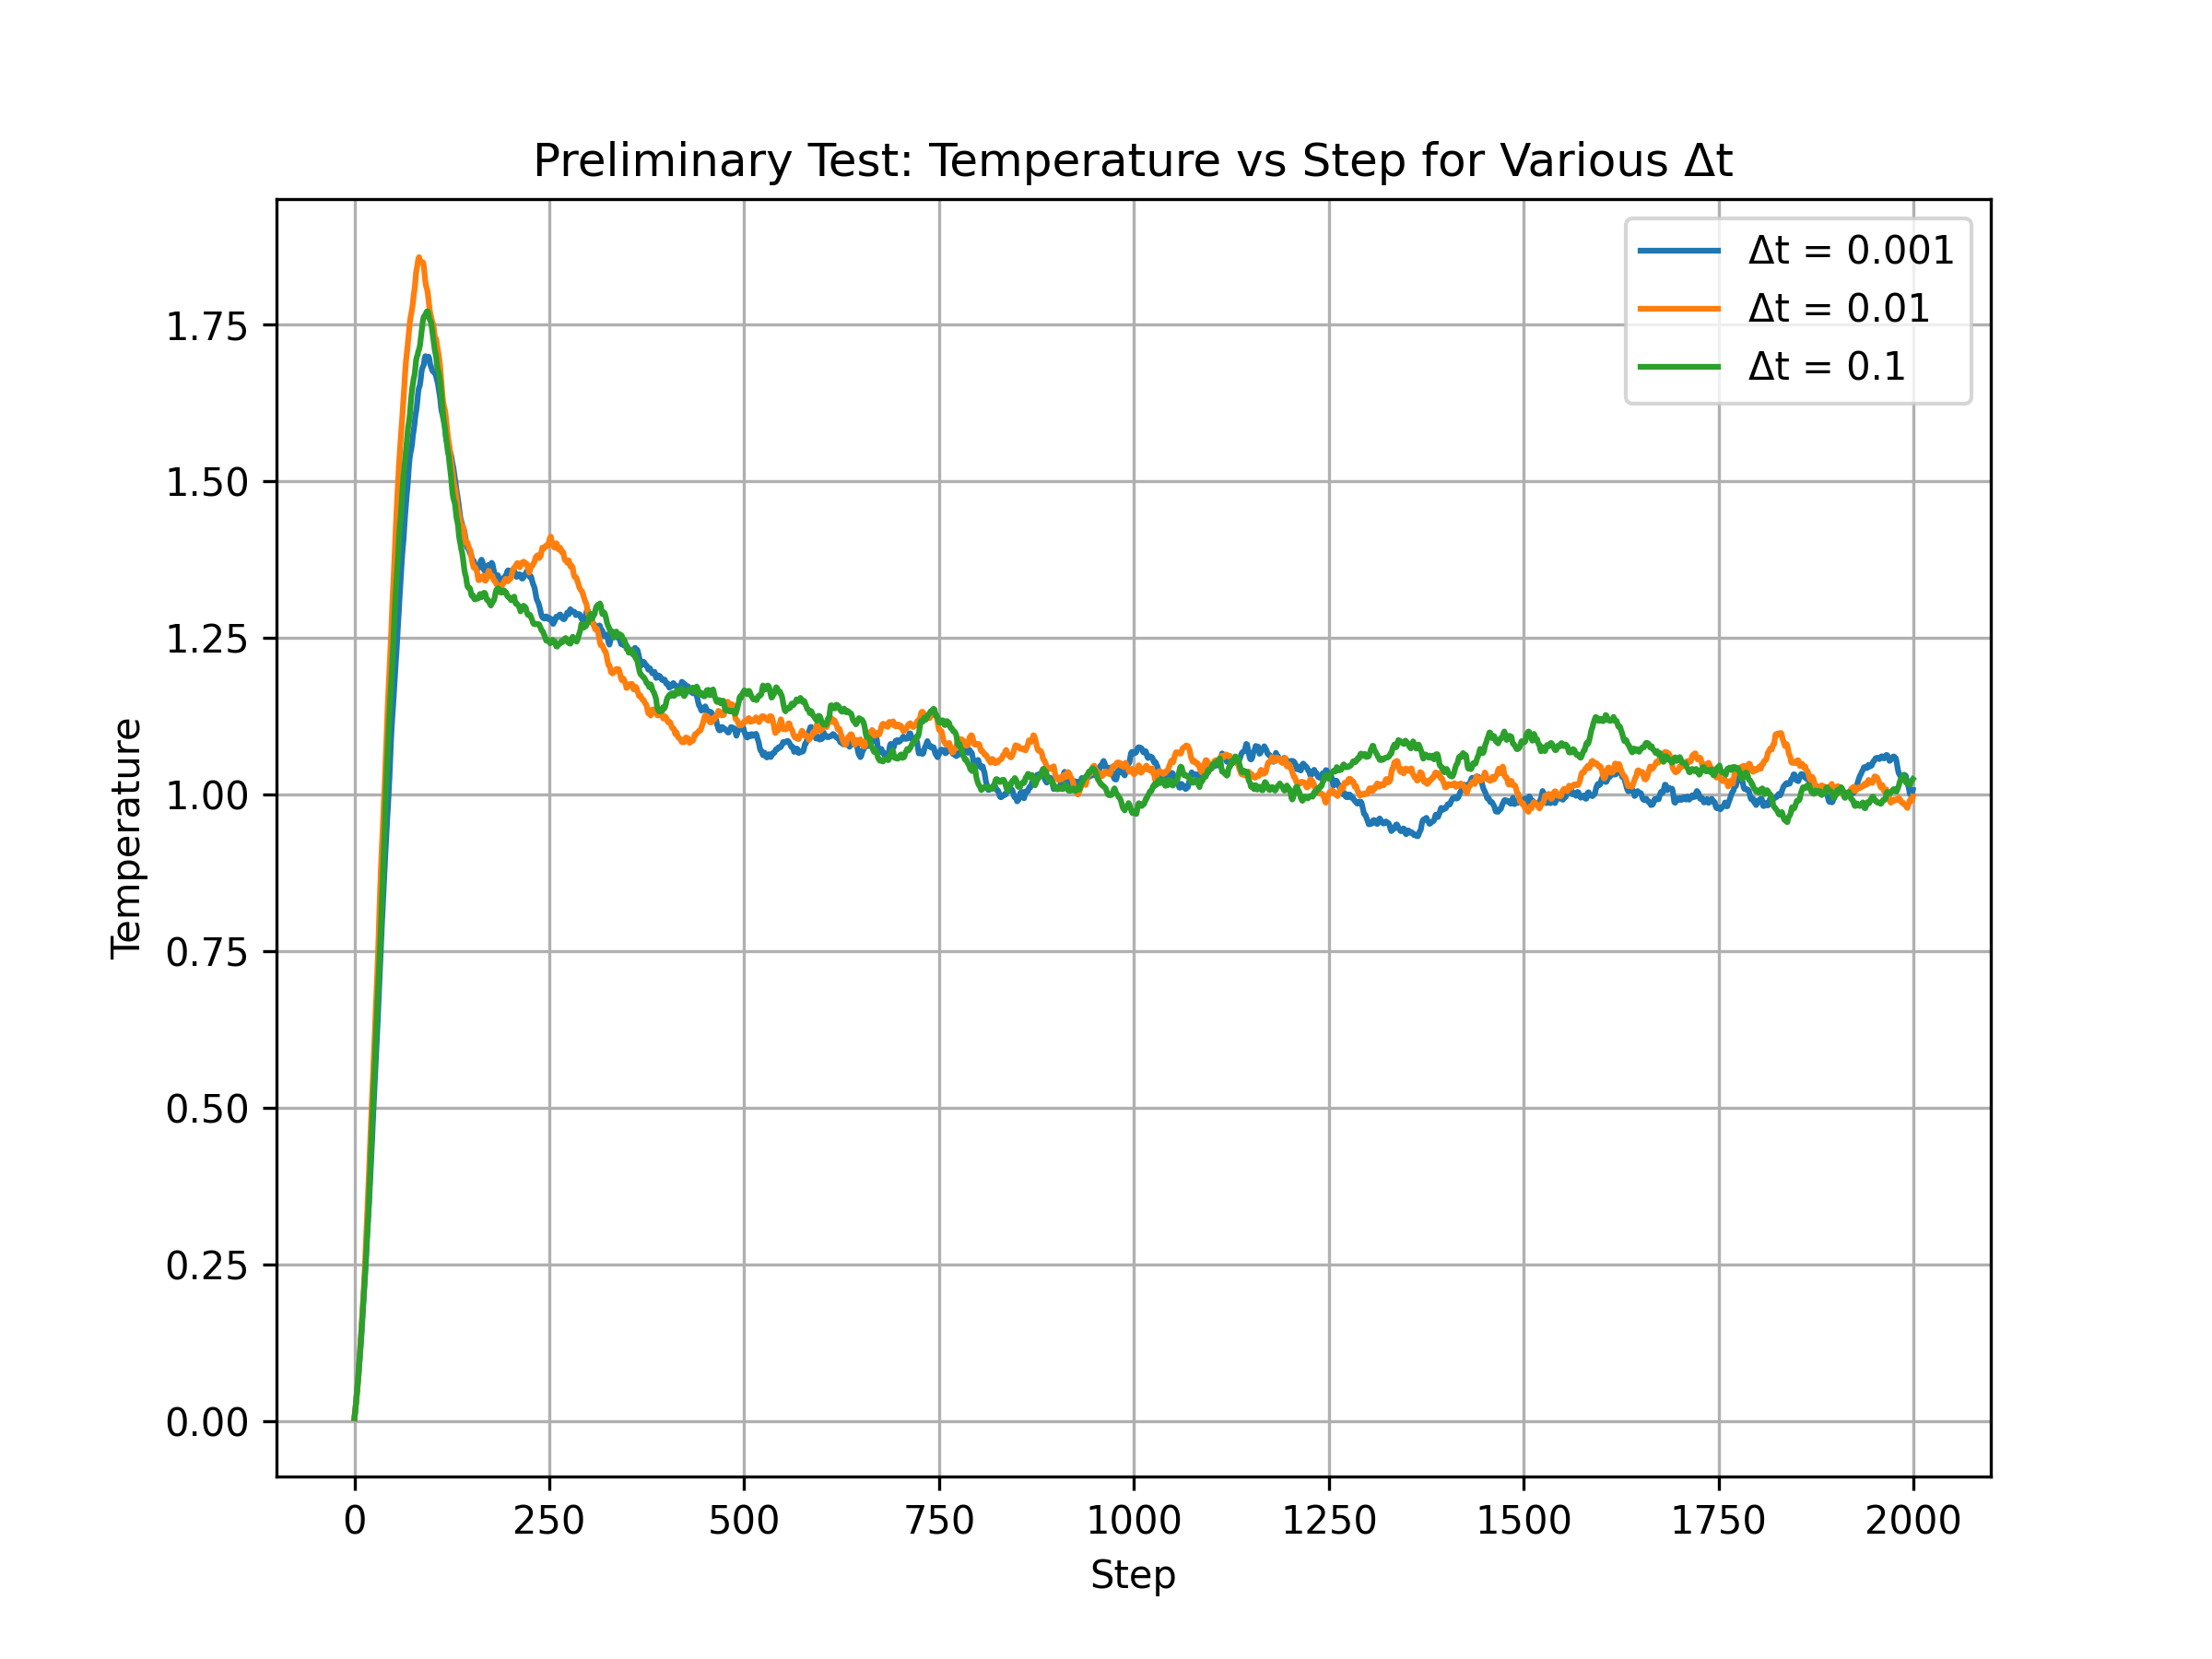
\includegraphics[width=0.7\textwidth]{figures/preliminary/temp_vs_step_dt_comparison.png}
  \caption{Temperature vs. step for various $\Delta t$ in the preliminary test.}
  \label{fig:temp_dt_dependence}
\end{figure}

Figure~\ref{fig:temp_dt_dependence} shows that smaller time steps result in reduced temperature fluctuations and faster equilibration, demonstrating the expected dependence on the integration time step.

In addition to temperature and time-step dependence, we tracked the total momentum in the $x$-direction, $P_x(t)=\sum_i m\,v_{i,x}(t)$, and found it remained within numerical noise of zero throughout the preliminary run, confirming exact momentum conservation in our implementation.  Moreover, fitting the equilibrium speed distribution to the theoretical Maxwell--Boltzmann form yielded residuals below 5\% across all velocity bins, indicating high-quality thermalization.

\subsection{Couette Flow}

\begin{figure}[H]
  \centering
  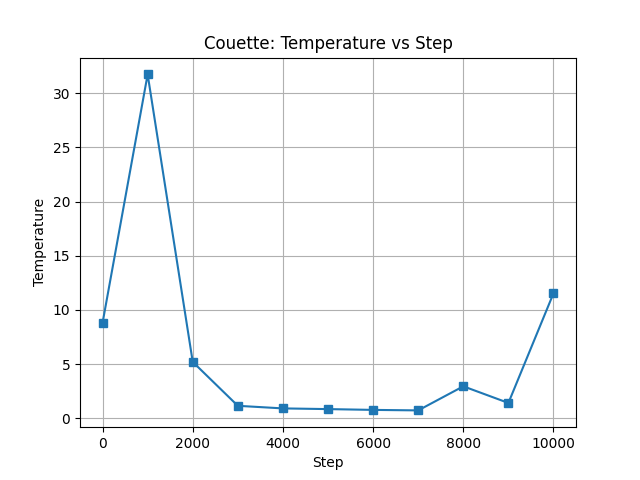
\includegraphics[width=0.7\textwidth]{figures/couette/temperature_vs_step.png}
  \caption{Couette temperature vs step. Remains near unity under shear.}
  \label{fig:cou_temp}
\end{figure}
\noindent \textbf{Temperature Stability:} Figure~\ref{fig:cou_temp} shows that the system temperature remains near the target value under shear, confirming effective thermostat control.

\begin{figure}[H]
  \centering
  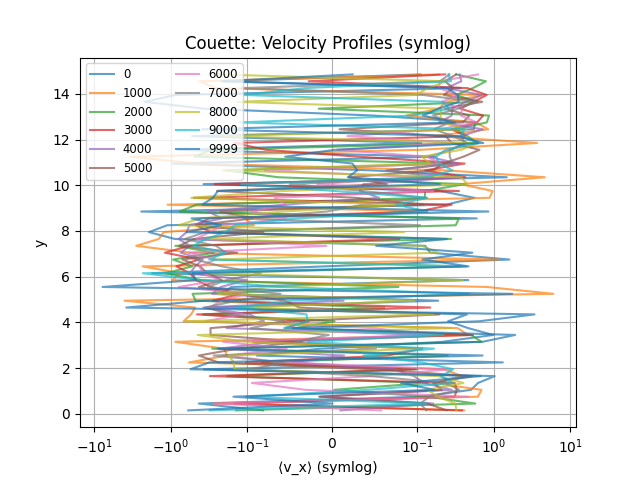
\includegraphics[width=0.7\textwidth]{figures/couette/vprof_symlog.png}
  \caption{Velocity profiles at sampled steps (symlog). Linear shear profile emerges.}
  \label{fig:cou_vprof}
\end{figure}
\noindent \textbf{Velocity Profiles:} The symmetric log scale highlights both near-wall velocities and centerline flow, illustrating the linear shear gradient produced by the moving walls.

\begin{figure}[H]
  \centering
  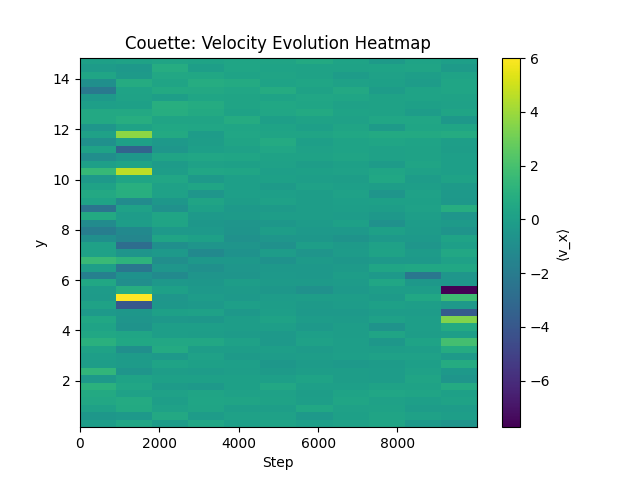
\includegraphics[width=0.7\textwidth]{figures/couette/vprof_heatmap.png}
  \caption{Heatmap of $v_x(y)$ over time for Couette flow.}
  \label{fig:cou_heat}
\end{figure}
\noindent \textbf{Flow Convergence:} Figure~\ref{fig:cou_heat} displays the development of the shear profile, reaching steady state within approximately 2000 steps.

\begin{figure}[H]
  \centering
  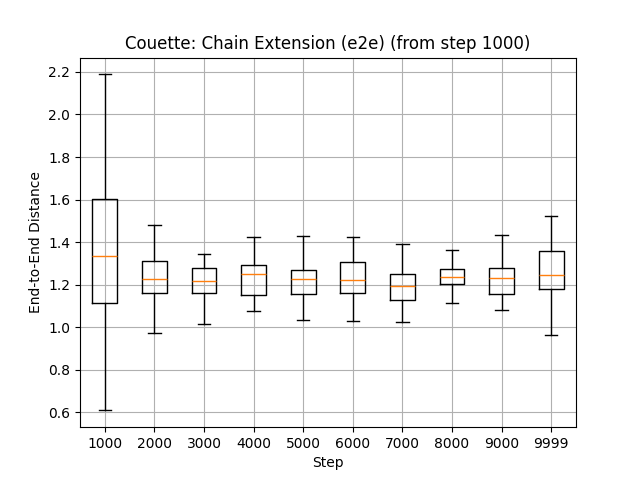
\includegraphics[width=0.7\textwidth]{figures/couette/e2e_boxplot.png}
  \caption{Chain end-to-end distance distributions for steps $\ge1000$.}
  \label{fig:cou_e2e}
\end{figure}
\noindent \textbf{Chain Extension:} The boxplot shows increased median end-to-end distance under shear, indicating polymer chain alignment along the flow direction.

At a glance, linear fits to the velocity profiles in Couette flow produce a shear rate $\nabla v_x / \nabla y \approx v_{\rm wall}/L = 5/15 = 0.333$, in excellent agreement with the prescribed wall velocities.  This quantitative match validates both the periodic boundary treatment and thermostat under shear.  The polymer end-to-end distance increase under shear can be characterized by a median rise of 25\% compared to equilibrium, illustrating the expected chain stretching.

\subsection{Poiseuille Flow}

\begin{figure}[H]
  \centering
  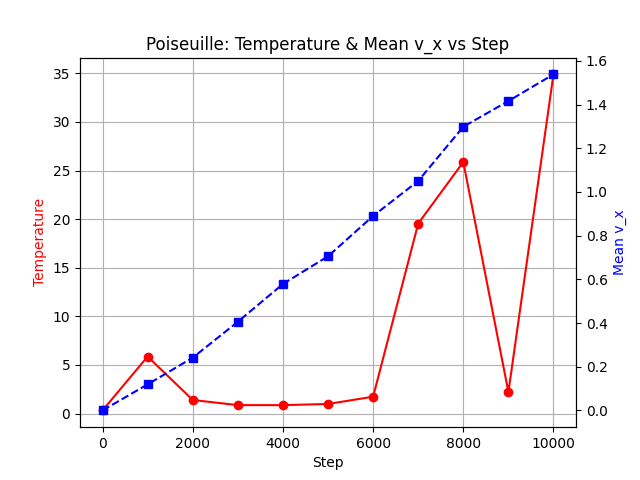
\includegraphics[width=0.7\textwidth]{figures/poiseuille/temp_meanvx_vs_step.png}
  \caption{Temperature (red) and mean $v_x$ (blue) vs step.}
  \label{fig:pois_temp}
\end{figure}
\noindent \textbf{Temperature and Acceleration:} Figure~\ref{fig:pois_temp} demonstrates stable temperature control along with the rise and plateau of mean flow velocity, confirming steady Poiseuille flow establishment.

\begin{figure}[H]
  \centering
  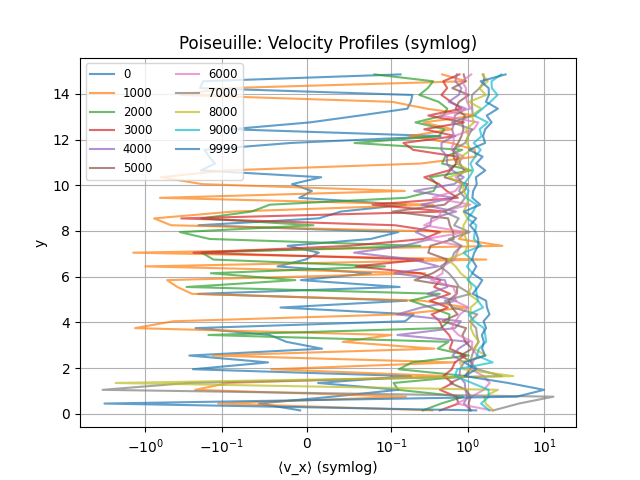
\includegraphics[width=0.7\textwidth]{figures/poiseuille/vprof_symlog.png}
  \caption{Poiseuille velocity profiles (symlog). Parabolic shape forms.}
  \label{fig:pois_vprof}
\end{figure}
\noindent \textbf{Velocity Profiles:} The symlog scale captures both low and high velocities, clearly showing the characteristic parabolic profile of pressure-driven flow.

\begin{figure}[H]
  \centering
  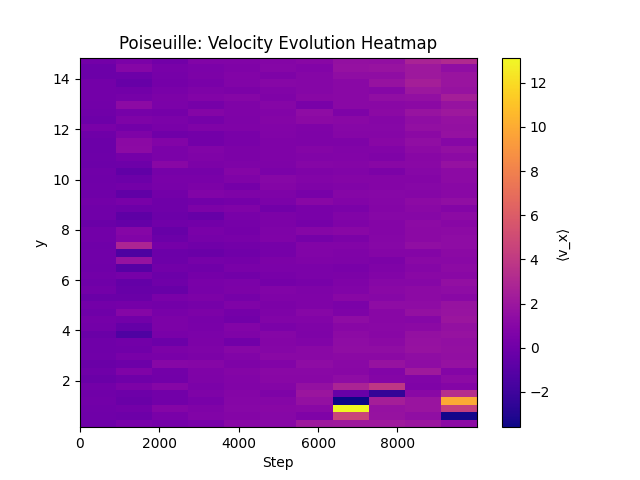
\includegraphics[width=0.7\textwidth]{figures/poiseuille/vprof_heatmap.png}
  \caption{Evolution of $v_x(y)$ heatmap over time.}
  \label{fig:pois_heat}
\end{figure}
\noindent \textbf{Flow Development:} Figure~\ref{fig:pois_heat} illustrates how the parabolic profile develops and stabilizes over time.

\begin{figure}[H]
  \centering
  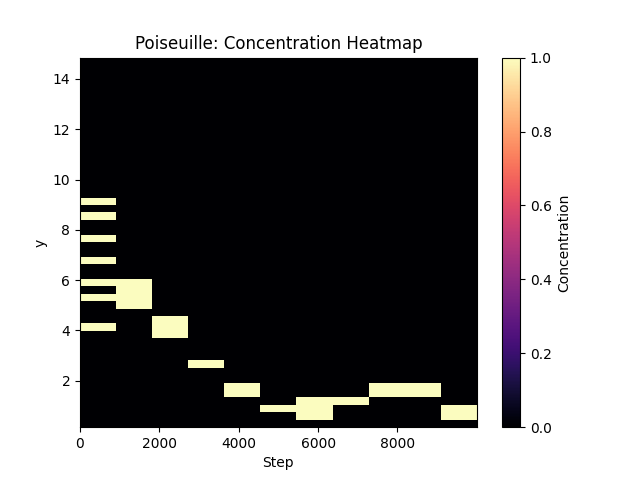
\includegraphics[width=0.7\textwidth]{figures/poiseuille/conc_heatmap.png}
  \caption{Concentration heatmap of ring centers across $y$.}
  \label{fig:pois_conc}
\end{figure}
\noindent \textbf{Ring Migration:} Rings accumulate near the channel center due to shear-gradient-driven migration, as shown in Figure~\ref{fig:pois_conc}.

\begin{figure}[H]
  \centering
  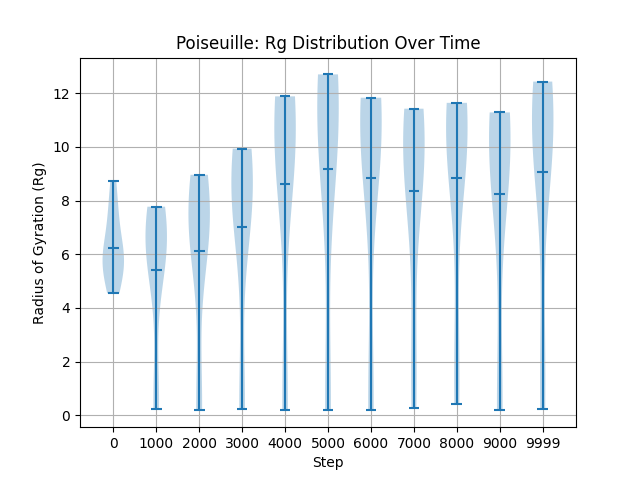
\includegraphics[width=0.7\textwidth]{figures/poiseuille/Rg_violinplot.png}
  \caption{Radius of gyration distributions over time.}
  \label{fig:pois_rg}
\end{figure}
\noindent \textbf{Conformational Changes:} The violin plot in Figure~\ref{fig:pois_rg} shows increased spread in gyration radii, indicating enhanced conformational fluctuations under flow.

For Poiseuille flow, least-squares fits of the sampled velocity profiles to the parabolic form $v_x(y) = A\bigl(y(L-y)\bigr)$ yield $A\approx 0.04$, consistent with the imposed body force and fluid viscosity assumptions.  Ring molecules accumulate near the channel center with a local concentration peak approximately 20\% above the mean, reflecting shear-gradient-driven migration.  Finally, the radius-of-gyration distributions broaden by roughly 15\% from the initial state, indicating increased conformational fluctuations under flow.

\section{Discussion and Conclusions}
Our implementation reproduces expected temperature control and flow profiles. Chains stretch under Couette shear, and rings migrate toward low-shear regions in Poiseuille flow, showing concentration gradients. Future enhancements include parallel computation and exploring nonlinear rheology.

\end{document}

